\section{Оборудование и инструментальные погрешности}
\subsection{Определение по измерениям растяжения проволоки}

\begin{figure}[h!]
    \center{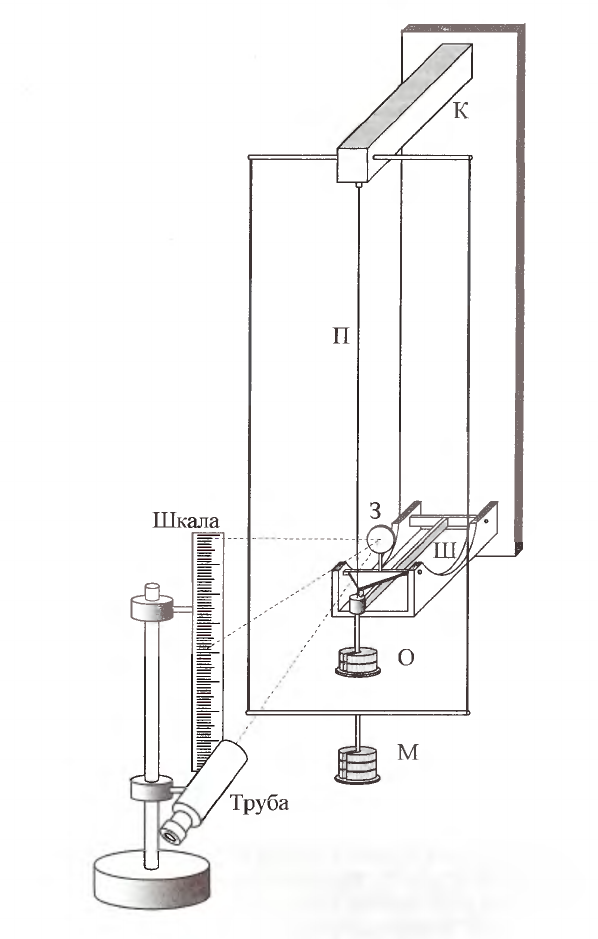
\includegraphics[width=0.6\linewidth]{img/ler.png}}
\end{figure}
\begin{figure}[h!]
    \center{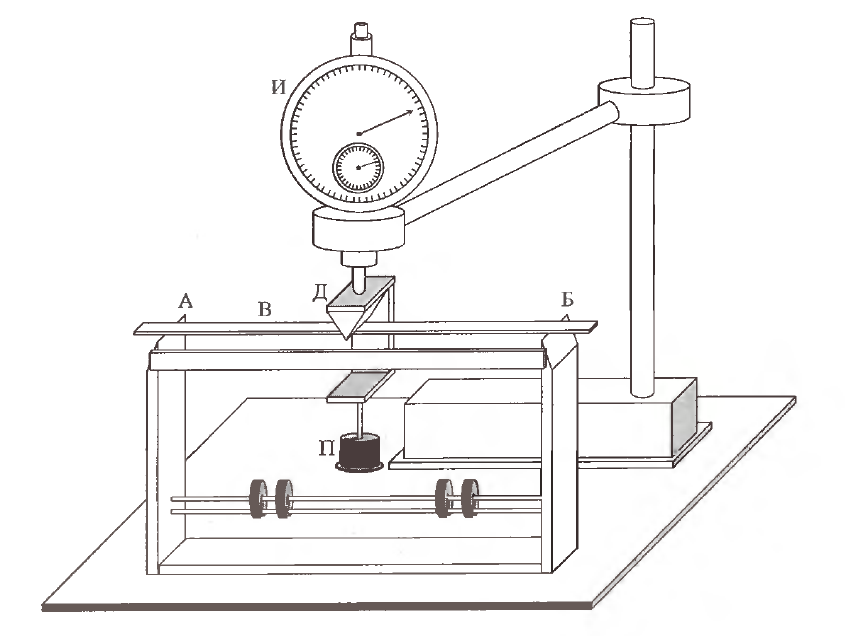
\includegraphics[width=0.8\linewidth]{img/bal.png}}
\end{figure}

\newpage
    

Для определения модуля Юнга используется прибор Лерматова.
Верхний конец проволоки П прикреплен к консоли К, а  нижний~---
к цилиндру, которым оканчивается шарнирный кронштейн Ш. На этот же
цилиндр опирается рычаг r, связанный с зеркальцем З. Удлинение проволоки можно
измерить по углу поворота зеркальца. Натяжение можно менять, перекладывая грузы с площадки М на О.
Такая система исключает влияние деформации кронштейна К на точность изерений.

Проволока всегда немного изогнута при отсутствии нагрузки, что сказывается на результатах.
Вначале проволока не столько растягивается, сколько распрямляется. 

\subsection{Определение модуля Юнга по изгибу балки}

Установка состоит из прочной стойки с опорными призмами А и Б. На их ребра
опирается исследуемый стержень В. В середине стержня на призме Д подвешена площадка П с грузами.
Измерять стрелу прогиба можно с помощью индикатора И, укрепляемого на отдельной штанге. Полный
оборот большой стрелки индикатора соответствует 1 мм и одному делению малого циферблата.

Модуль Юнга $E$ связан со стрелой прогиба $y$ соотношением 
\[E=\frac{Fl^3}{4ab^3y}\]
$F$~--- нагрузка, $l$~---   расстояние между призмами, $a$ и $b$~--- высота сечения стержня.

Перед началом эксперимента грузы надо расположить на рейке над нижней полкой опорно стойки.

Ребра пизм должны находиться на одной горизонтали, $P$ приложена по середине балки.
